%Beamer class
\pdfminorversion=7
\documentclass{beamer}

\usepackage[czech]{babel}
\usepackage[utf8]{inputenc}
\usepackage[T1]{fontenc}
\usepackage{tgheros}
\usepackage{tgcursor}
\usepackage{array}
\usepackage{color}
\usepackage{hyperref}
\usepackage{fancyvrb} % pro verbatim
\usepackage{graphicx}
\usepackage{tikz}

\usetheme{AnnArbor}
\usecolortheme{crane}
\setbeamerfont{description item}{series=\bfseries}


\title[Pravidla návrhu DPS]{Základní pravidla návrhu DPS}
\subtitle[KEO]{\texorpdfstring{Konstrukce a realizace elektronických obvodů}{Konstrukce a realizace elektronickych obvodu}}
\author[Brejcha]{\texorpdfstring{Michal Brejcha\newline\url{brejcmic@fel.cvut.cz}}{Michal Brejcha}}
\institute[ČVUT]{ČVUT v Praze, FEL}
\date[Praha, 2026]{Praha, 2026}

%------------------------------------------------------------------------------
%Konstanty a definice
%------------------------------------------------------------------------------
\newtheorem{myDef}{}
\newcommand{\kicadVersion}{10.0}

\begin{document}
%------------------------------------------------------------------------------
%Uvodni slajd
%------------------------------------------------------------------------------
\frame{\titlepage}

\begin{frame}
\frametitle{Obsah} 
\tableofcontents
\end{frame}

\AtBeginSection[]
{
  \begin{frame}
    \frametitle{Téma}
    \tableofcontents[currentsection]
  \end{frame}
}

%------------------------------------------------------------------------------
% Fyzická skladba DPS
%------------------------------------------------------------------------------
\section{\texorpdfstring{Fyzická skladba DPS}{Fyzicka skladba DPS}}
%------------------------------------------------------------------------------
\begin{frame}[t]{Stackup: nejde pouze o počet vrstev}
	\begin{itemize}
		\item \textbf{Stackup} určuje pořadí měděných vrstev, jejich funkci a tloušťky izolačních materiálů mezi nimi.
		\item \textbf{SIG}: signály; \textbf{PWR}: napájení; \textbf{GND}: referenční vodič a návratová cesta proudu.
		\item Zápis \textbf{SIG + PWR} označuje jednu společnou vrstvu pro signálové trasy a rozvod napájení, nikoli dvě vrstvy.
		\item Pořadí v obrázcích čteme \textbf{shora dolů}. Čísla L1--L4 odpovídají pořadí měděných vrstev.
	\end{itemize}
	\begin{block}{Základní doporučení}
	Signál potřebuje blízkou a souvislou referenční plochu. Důležité jsou i rychlost hran signálu a délka vedení, nejen hodinová frekvence.
	\end{block}
	\vfill
	{\tiny Zdroj doporučení: [1, 5, 6]. Úplný seznam zdrojů je na konci prezentace.}
\end{frame}

%------------------------------------------------------------------------------
\begin{frame}[t]{Dvě vrstvy: (SIG + PWR) / GND}
	\small
	{\centering
		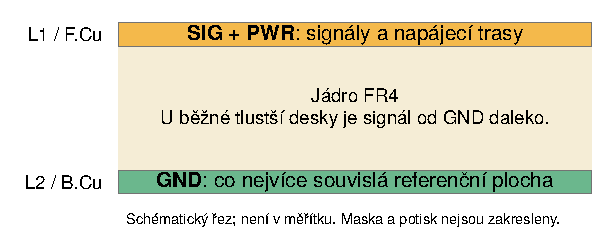
\includegraphics[width=0.98\linewidth,height=0.59\textheight,keepaspectratio]{obr/stackup_2layer.pdf}\par}
	\medskip
	Signály a napájení veďte převážně na L1; protější L2 ponechte co nejvíce souvislou jako návratovou cestu GND.
	\vfill
	{\tiny Zdroj doporučení: [1] Z. Peterson.}
\end{frame}

%------------------------------------------------------------------------------
\begin{frame}[t]{Dvě vrstvy: výhody a omezení}
	\begin{itemize}
		\item \textbf{Výhody:} jednoduchá a levná výroba; přehledná návratová cesta oproti desce s rozdělenou zemí na obou stranách.
		\item \textbf{Nevýhody:} méně prostoru pro signály a napájení; u běžné tloušťky 1,6 mm je protější GND vzdálená, takže vazba a řízení impedance jsou horší než u vhodné čtyřvrstvé desky.
		\item \textbf{Použití:} jednodušší obvody s krátkými vedeními. Spodní GND co nejméně přerušovat; trasy přes celou spodní stranu mohou rozříznout návratovou cestu.
	\end{itemize}
	\vfill
	{\tiny Zdroj doporučení: [1] Z. Peterson.}
\end{frame}

%------------------------------------------------------------------------------
\begin{frame}[t]{Čtyři vrstvy: SIG / GND / PWR / SIG}
	\small
	{\centering
		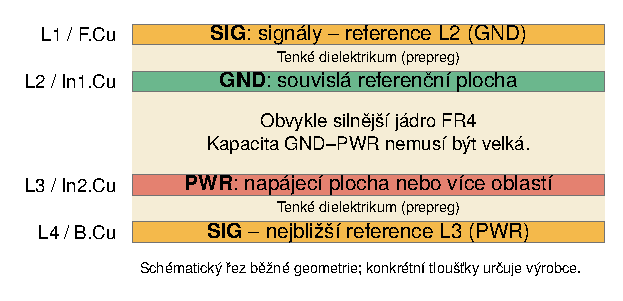
\includegraphics[width=0.98\linewidth,height=0.61\textheight,keepaspectratio]{obr/stackup_4layer_power.pdf}\par}
	\medskip
	L1 má referenci GND, zatímco nejbližší referencí pro L4 je PWR. Právě tento rozdíl ovlivňuje vedení rychlých signálů.
	\vfill
	{\tiny Zdroj doporučení: [2] Z. Peterson.}
\end{frame}

%------------------------------------------------------------------------------
\begin{frame}[t]{SIG / GND / PWR / SIG: výhody a omezení}
	\begin{itemize}
		\item \textbf{Výhody:} dvě signálové vrstvy a samostatný rozvod napájení; horní signály mají blízkou GND.
		\item \textbf{Nevýhody:} spodní signály mají nejbližší referenci PWR. Rozdělení napájecí plochy a změna reference při přechodu vrstev komplikují návrat proudu.
		\item \textbf{Použití:} rychlé signály přednostně na L1 nad GND. Plná PWR může být referencí pro L4, ale je nutné vyřešit návaznost návratového proudu na GND.
	\end{itemize}
	\vfill
	{\tiny Zdroj doporučení: [2] Z. Peterson.}
\end{frame}

%------------------------------------------------------------------------------
\begin{frame}[t]{Čtyři vrstvy se dvěma plochami GND}
	\small
	{\centering
		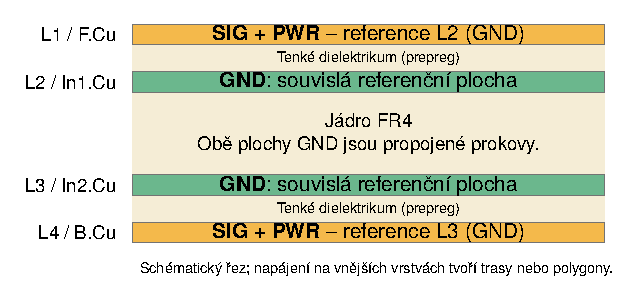
\includegraphics[width=0.98\linewidth,height=0.61\textheight,keepaspectratio]{obr/stackup_4layer_gnd.pdf}\par}
	\medskip
	Napájení lze rozvádět na jedné nebo obou vnějších vrstvách. Dvě vnitřní GND plochy ponechte souvislé a vzájemně je propojte.
	\vfill
	{\tiny Zdroj doporučení: [3] Z. Peterson.}
\end{frame}

%------------------------------------------------------------------------------
\begin{frame}[t]{Dvě plochy GND: výhody a omezení}
	\begin{itemize}
		\item \textbf{Výhody:} obě vnější vrstvy mají blízkou referenci GND; vnitřní plochy oddělují signály na protilehlých stranách.
		\item \textbf{Nevýhody:} napájení sdílí prostor se signály, není k dispozici samostatná PWR vrstva. Pro větší proudy a mnoho napěťových úrovní (zdrojů) může chybět místo.
		\item \textbf{Doporučení:} vhodný výchozí stackup pro běžnou čtyřvrstvou digitální desku. GND plochy propojit; u přechodu signálu vložit blízký GND prokov.
	\end{itemize}
	\vfill
	{\tiny Zdroj doporučení: [3] Z. Peterson.}
\end{frame}

%------------------------------------------------------------------------------
\begin{frame}[t]{Návratová cesta při změně signálové vrstvy}
	\begin{itemize}
		\item U rychlých změn proudu se návratový proud soustřeďuje do blízké referenční plochy pod trasou.
		\item \textbf{GND → GND:} při přechodu L1 $\leftrightarrow$ L4 propojte obě referenční plochy GND prokovem poblíž signálového prokovu.
		\item \textbf{GND → PWR:} samotný GND prokov nestačí. Přechod návratového proudu vyžaduje vhodnou vazbu mezi PWR a GND, např. blízký blokovací kondenzátor s krátkým připojením.
		\item Signál neveďte přes mezeru, výřez nebo rozhraní různých napětí v jeho referenční ploše.
	\end{itemize}
	\begin{block}{Výhoda dvou GND vrstev}
	Návratovou cestu lze při přechodu jednodušeji navázat GND prokovem. GND a PWR se naopak nesmějí spojit přímým prokovem.
	\end{block}
	\vfill
	{\tiny Zdroj doporučení: [4, 5, 7, 9] Peterson, Bogatin, Kay, Salmony.}
\end{frame}

%------------------------------------------------------------------------------
\begin{frame}[t]{Bez GND prokovů: přerušená návaznost reference}
	\footnotesize
	{\centering
	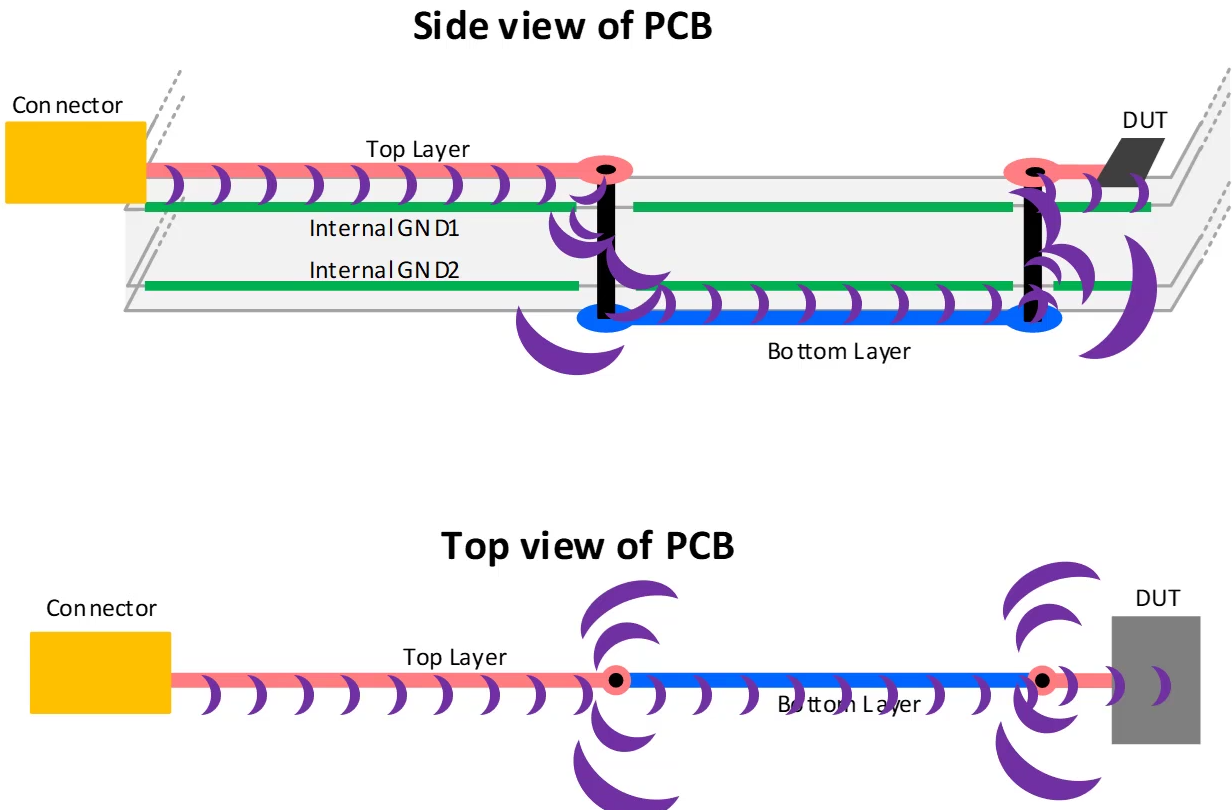
\includegraphics[width=.98\linewidth,height=.58\textheight,keepaspectratio]{obr/wave_guide_no_vias.png}\par}
	\footnotesize
	\begin{itemize}
		\item Nahoře boční pohled, dole pohled shora. Signál mění vrstvu, ale mezi oběma GND plochami chybí blízké propojení.
		\item Fialové značky ilustrují pole: u přechodů se rozprostírá do okolí.
	\end{itemize}
	\vfill
	{\tiny Obrázek a princip: [7] A. Kay (Texas Instruments), snímek 9.}
\end{frame}

%------------------------------------------------------------------------------
\begin{frame}[t]{GND $\rightarrow$ GND: návrat přes blízký prokov}
	\small
	{\centering
	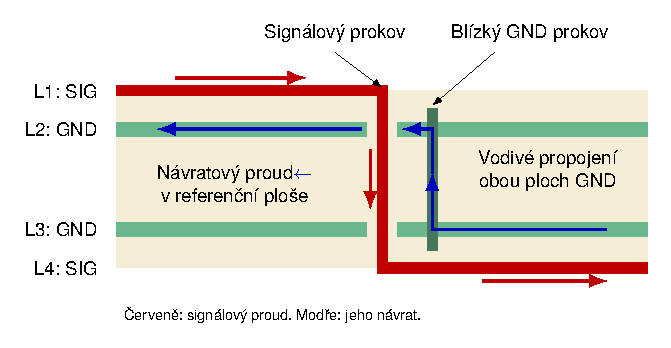
\includegraphics[width=\linewidth,height=.51\textheight,keepaspectratio]{obr/return_gnd.pdf}\par}
	\begin{itemize}
		\item Signál přechází z L1 na L4; návrat se přesouvá z L3 na L2 po \textbf{blízkém GND prokovu}.
		\item Čím vzdálenější je návratový prokov, tím větší je proudová smyčka. Signálový prokov se s GND plochami nespojuje.
	\end{itemize}
	\vfill
	{\tiny Zdroj doporučení: [7, 9] A. Kay (TI), P. Salmony (Phil's Lab).}
\end{frame}

%------------------------------------------------------------------------------
\begin{frame}[t]{GND prokovy: boční a horní pohled}
	\footnotesize
	{\centering
	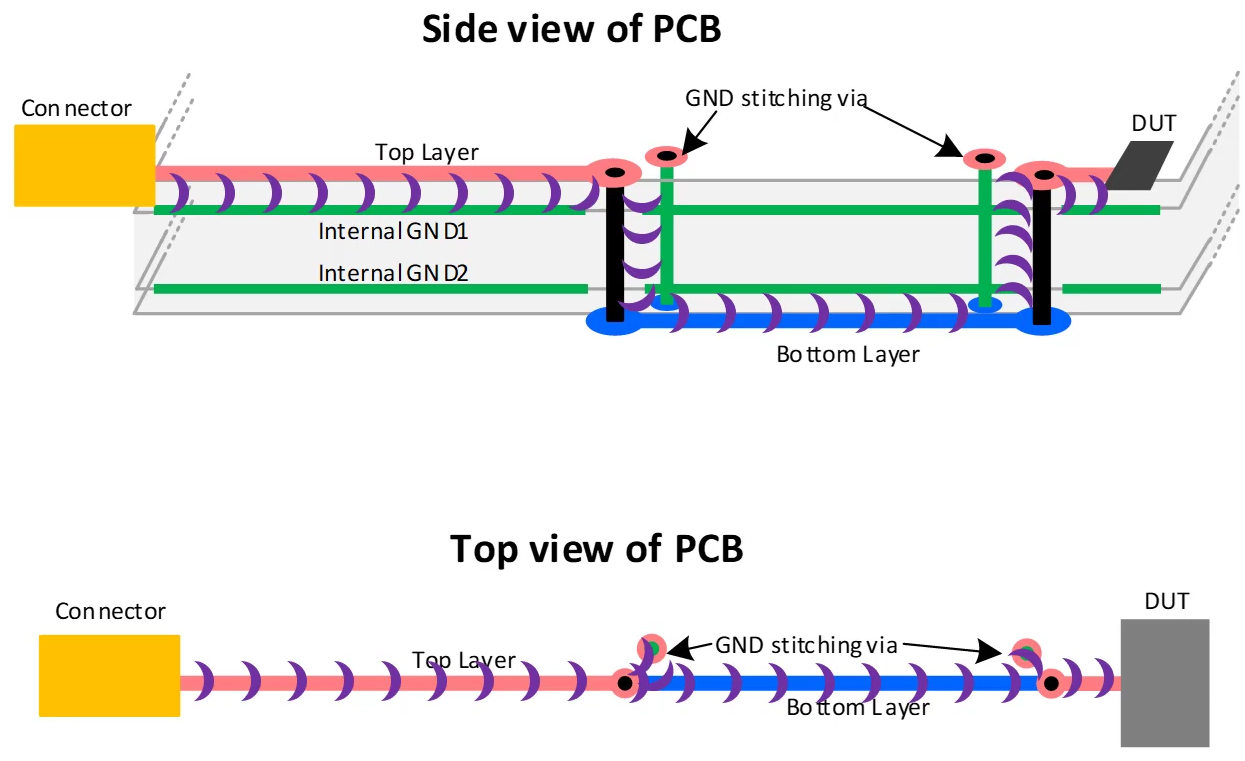
\includegraphics[width=.98\linewidth,height=.58\textheight,keepaspectratio]{obr/wave_guide_gnd_vias.png}\par}
	\footnotesize
	\begin{itemize}
		\item Zelené GND prokovy vedle černých signálových prokovů propojují obě vnitřní GND plochy.
		\item Návrat má blízkou cestu při obou změnách signálové vrstvy; pole se drží blíže k vedení a referenci.
	\end{itemize}
	\vfill
	{\tiny Obrázek a princip: [7] A. Kay (Texas Instruments), snímek 8.}
\end{frame}

%------------------------------------------------------------------------------
\begin{frame}[t]{Ukázka v KiCadu: GND vedle signálového prokovu}
	\small
	\begin{columns}[T,onlytextwidth]
		\begin{column}{.46\textwidth}
			\begin{itemize}
				\item \textbf{SIG}: prokov mění signálovou vrstvu; červená trasa je F.Cu, modrá B.Cu.
				\item \textbf{GND}: sousední prokov propojuje vnitřní referenční plochy L2 a L3.
				\item GND prokov přidat přímo k přechodu, ne až na vzdálený okraj desky. Dodržet izolační odstupy.
			\end{itemize}
		\end{column}
		\begin{column}{.52\textwidth}
			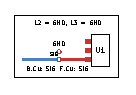
\includegraphics[width=\linewidth]{obr/layout_gnd.pdf}
			{\scriptsize Export z KiCadu 10, pohled shora. Vnitřní měděné plochy jsou skryté. U1 je pouze výukový model.}
		\end{column}
	\end{columns}
	\vfill
	{\tiny Zdroj doporučení: [7, 9] A. Kay (TI), P. Salmony (Phil's Lab).}
\end{frame}

%------------------------------------------------------------------------------
\begin{frame}[t]{GND $\rightarrow$ PWR: návrat přes kondenzátor}
	\small
	{\centering
	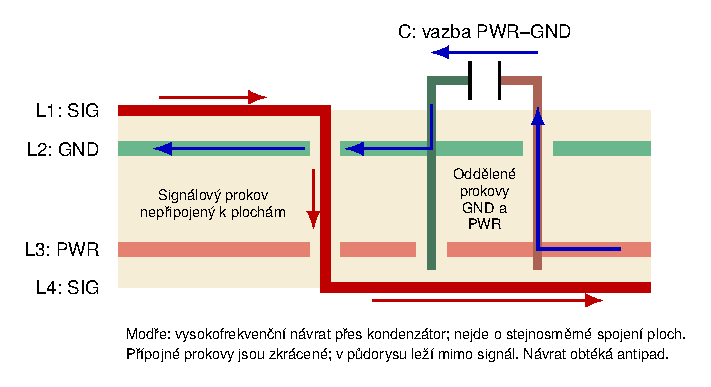
\includegraphics[width=\linewidth,height=.51\textheight,keepaspectratio]{obr/return_cap.pdf}\par}
	\begin{itemize}
		\item Návrat mezi různými referencemi potřebuje \textbf{nízkoimpedanční kapacitní vazbu} poblíž přechodu.
		\item GND a PWR se nesmějí spojit prokovem! Kondenzátor je \textbf{mezi PWR a GND}, nikoli v sérii se signálem.
	\end{itemize}
	\vfill
	{\tiny Zdroj doporučení: [4, 7, 9] Z. Peterson, A. Kay (TI), P. Salmony.}
\end{frame}

%------------------------------------------------------------------------------
\begin{frame}[t]{GND $\rightarrow$ PWR: boční a horní pohled}
	\footnotesize
	{\centering
	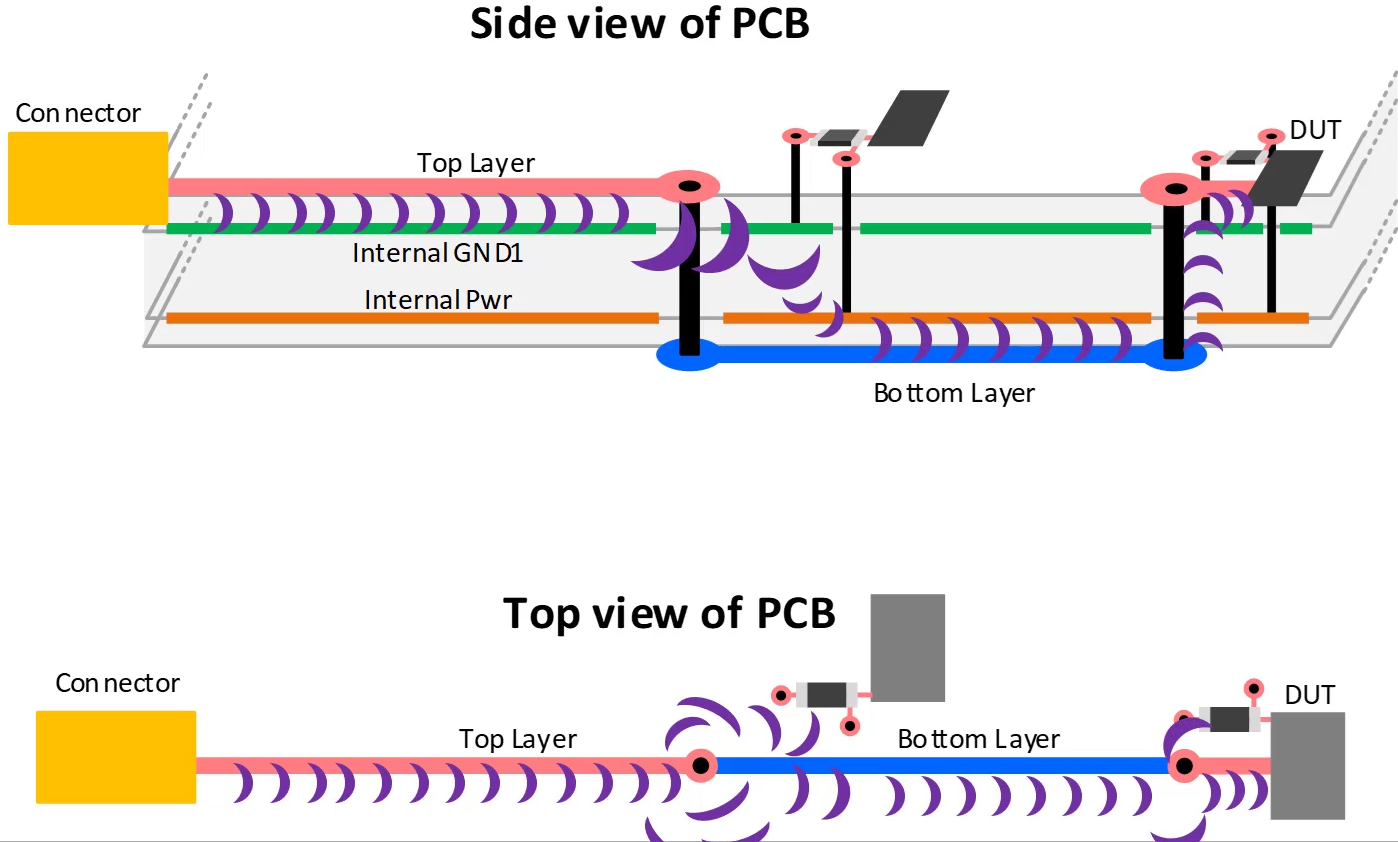
\includegraphics[width=.98\linewidth,height=.58\textheight,keepaspectratio]{obr/wave_guide_capacitors.png}\par}
	\footnotesize
	\begin{itemize}
		\item Zelená plocha je GND, oranžová PWR. Kondenzátory u přechodů zajišťují kapacitní vazbu mezi referencemi.
		\item Vpravo tuto úlohu plní blokování u součástky (DUT). GND a PWR nejsou spojeny přímo; kondenzátory nejsou v signálové trase.
	\end{itemize}
	\vfill
	{\tiny Obrázek a princip: [7] A. Kay (Texas Instruments), snímek 12.}
\end{frame}

%------------------------------------------------------------------------------
\begin{frame}[t]{Ukázka v KiCadu: blokování u přechodu signálu}
	\small
	\begin{columns}[T,onlytextwidth]
		\begin{column}{.46\textwidth}
			\begin{itemize}
				\item \textbf{C1} je mezi napájením U1 a GND. Připojení plošek k jejich prokovům je krátké a široké.
				\item Blízký blokovací kondenzátor součástky může současně navázat návrat u \textbf{SIG prokovu}.
				\item Musí patřit ke \textbf{stejnému napájení}, které tvoří referenci L3. Vzdálený kondenzátor tuto úlohu nemusí splnit.
			\end{itemize}
		\end{column}
		\begin{column}{.52\textwidth}
			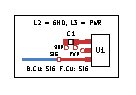
\includegraphics[width=\linewidth]{obr/layout_cap.pdf}
			{\scriptsize Export z KiCadu 10. L2 = GND, L3 = PWR; obě plochy jsou skryté. U1 má pouze modelové vývody.}
		\end{column}
	\end{columns}
	\vfill
	{\tiny Zdroj doporučení: [7--9] A. Kay (TI), D. L. Jones, P. Salmony.}
\end{frame}

%------------------------------------------------------------------------------
\begin{frame}[t]{Tloušťky dielektrika a napájení}
	\begin{itemize}
		\item U čtyřvrstvé desky požadujte blízké dvojice \textbf{L1--L2} a \textbf{L3--L4}; běžná stavba má tenké prepregy a silnější středové jádro.
		\item Menší vzdálenost signálu od reference pomáhá omezit plochu proudové smyčky. Impedanci ale určuje i šířka a tloušťka mědi a vlastnosti dielektrika.
		\item Vzdálené plochy PWR a GND mají malou vzájemnou kapacitu. \textbf{Samostatná PWR vrstva nenahrazuje blokovací kondenzátory.}
		\item Konkrétní tloušťky, materiály a dostupné varianty ověřte u výrobce \textbf{před návrhem impedančně řízených spojů}.
	\end{itemize}
	\vfill
	{\tiny Zdroj doporučení: [2, 6] Z. Peterson, Phil's Lab.}
\end{frame}

%------------------------------------------------------------------------------
\begin{frame}[t]{Jak zvolit výchozí skladbu?}
	\small
	\begin{description}
		\item[(SIG + PWR) / GND] Pro jednoduché, méně husté desky. Prioritou je zachování GND, ne zaplnění obou stran signály.
		\item[SIG / GND / PWR / SIG] Když pomůže samostatná napájecí plocha a nejdůležitější signály zůstanou nad GND. Není to automaticky chybné řešení, ale spodní signály vyžadují pozornost.
		\item[(SIG + PWR) / GND / GND / (SIG + PWR)] Vhodný výchozí kompromis pro digitální signály na obou stranách. Napájení řešte dostatečně širokými trasami či polygony.
	\end{description}
	\begin{block}{Neexistuje jedna skladba pro všechny desky}
	Rozhodují proudy, napětí, rychlost hran, hustota zapojení a požadavky na rušení. Pokud se napájení a signály nevejdou bez porušení návratových cest, zvažte více vrstev.
	\end{block}
	\vfill
	{\tiny Zdroj doporučení: [1--6]. Výukové shrnutí; úplný seznam zdrojů následuje na konci.}
\end{frame}

%------------------------------------------------------------------------------
\section{\texorpdfstring{Přerušení zpětné cesty}{Preruseni zpetne cesty}}
%------------------------------------------------------------------------------

%------------------------------------------------------------------------------
\section{\texorpdfstring{Referenční zdroje}{Referencni zdroje}}
%------------------------------------------------------------------------------
\begin{frame}[t]{Zdroje (1/2): skladba DPS a referenční plochy}
	\small
	\begin{enumerate}
		\item Z. Peterson: \href{https://resources.altium.com/p/understanding-ground-planes-your-two-layer-pcb}{Understanding 2-Layer PCB Ground Planes}.
		\item Z. Peterson: \href{https://resources.altium.com/p/right-way-use-power-planes-4-layer-pcb-stackup}{The Right Way to Use Power Planes in a 4-Layer PCB Stackup}.
		\item Z. Peterson: \href{https://resources.altium.com/p/two-alternative-4-layer-pcb-stackups-50-ohms-impedance}{Two 4 Layer PCB Stackups With 50 Ohms Impedance}.
		\item Z. Peterson: \href{https://resources.altium.com/p/should-you-use-your-power-plane-as-a-return-path}{Should You Use Your PCB Power Plane as a Return Path?}
		\item E. Bogatin: \href{https://www.signalintegrityjournal.com/articles/2982-the-case-for-split-ground-planes}{The Case for Split Ground Planes}, Signal Integrity Journal, 2023.
		\item Phil's Lab: \href{https://resources.altium.com/p/pcb-stackup-basics}{PCB Stackup Basics}, Altium.
	\end{enumerate}
	\medskip
	{\scriptsize Čísla v drobných odkazech na slajdech odpovídají tomuto seznamu.}
\end{frame}

%------------------------------------------------------------------------------
\begin{frame}[t]{Zdroje (2/2): návratový proud a blokování}
	\small
	\begin{enumerate}
		\setcounter{enumi}{6}
		\item Art Kay: \href{https://www.ti.com/video/6307562268112}{PCB Trace as a Wave Guide}, TI Precision Labs -- ADCs, Texas Instruments. \href{https://www.ti.com/content/dam/videos/external-videos/zh-tw/9/3816841626001/6307562268112.mp4/subassets/pcb-trace-as-wave-guide-presentation-quiz.pdf}{Podklad k videu}, snímky 8, 9 a 12. Použity uživatelem dodané snímky s bočním a horním pohledem.
		\item David L. Jones: \href{https://www.scs.stanford.edu/~zyedidia/docs/pcb/pcb_tutorial.pdf}{\textit{PCB Design Tutorial}}, revize A, 29. 6. 2004, str. 19--20: Good Bypassing, High Frequency Design Techniques. Veřejná kopie na webu Stanford University.
		\item Phil Salmony (Phil's Lab): \href{https://resources.altium.com/p/vias-101}{Vias 101: Standards, Sizing, and Spacing}, Altium; části Transfer Vias a Placement.
	\end{enumerate}
	\medskip
	{\scriptsize Ostatní obrázky jsou vlastní česká schémata nebo vlastní exporty výukových desek z KiCadu 10. Editovatelné předlohy i PDF jsou v \texttt{obr/}. Řezy nejsou v měřítku; ukázkové desky nejsou výrobním návrhem. Z Jonesova staršího podkladu přebíráme zásady blokování, nikoli obecné doporučení dělit zemní plochy.}
\end{frame}


\end{document}
